\model{Linked List}

A more flexible strategy for storing a list of numbers in memory is to use \emph{pointers}.
A pointer is a memory address for the next item in the list.

\begin{center}
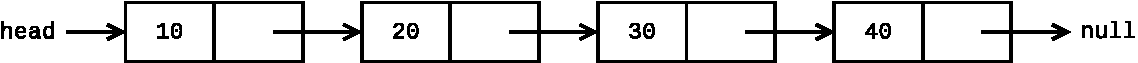
\includegraphics[width=0.85\linewidth]{linked1.pdf}
\end{center}

For example, the list \pyth{[10, 20, 30, 40]} could be stored in memory this way:

\setlength{\defaultwidth}{1em}

\begin{center}
\renewcommand{\arraystretch}{1.8}
\begin{tabular}{rccccccccccccc}
\textit{Address:~~} &  & 74 & 75 & 76 & 77 & 78 & 79 & 80 & 81 & 82 & 83 &
\\ \cline{2-13}
\textit{Value:~~} &
\multicolumn{1}{c|}{~~$\cdots$~~} &
\multicolumn{1}{c|}{30} &
\multicolumn{1}{c|}{78} &
\multicolumn{1}{c|}{10} &
\multicolumn{1}{c|}{80} &
\multicolumn{1}{c|}{40} &
\multicolumn{1}{c|}{0} &
\multicolumn{1}{c|}{20} &
\multicolumn{1}{c|}{74} &
\multicolumn{1}{c|}{} &
\multicolumn{1}{c|}{} &
~~$\cdots$~~
\\ \cline{2-13}
\textit{Index:~~} &
& \ans{2}
& \ans{}
& \ans{0}
& \ans{}
& \ans{3}
& \ans{}
& \ans{1}
& \ans{}
& \ans{}
& \ans{}
&
\end{tabular}
\end{center}

We use the memory address 0 to represent the \emph{null pointer}.


\quest{10 min}


\Q How many memory cells are needed for each list item?

\begin{answer}[2em]
Two cells: one for the number, and one for the pointer.
\end{answer}


\Q In the diagram above, write the index of each list item below the corresponding memory cell. Note there are only four items in the list, so you should only have four indexes.

\vspace{1em}


\Q Is there a relationship between the index and the corresponding memory address? Why or why not?

\begin{answer}
There is none; elements can be stored in memory in any order.
\end{answer}


\Q What is the purpose of the null pointer?

\begin{answer}
To know where the list ends.
\end{answer}


\Q The statement \pyth{lucky.insert(2, 25)} changes the list to \pyth{[10, 20, 25, 30, 40]}.
In \ref{\currfilename}, change the values of memory cells \pyth{81}, \pyth{82}, and \pyth{83} to perform this insertion.

\vspace{-1ex}
\begin{center}
\renewcommand{\arraystretch}{1.8}
\begin{tabular}{ccc}
81 & 82 & 83 \\ \hline
 \multicolumn{1}{|c|}{\ans[2em]{82}}
& \multicolumn{1}{c|}{\ans[2em]{25}}
& \multicolumn{1}{c|}{\ans[2em]{74}}
\\ \hline
\end{tabular}
\end{center}
\vspace{1ex}


\Q What memory operations does it take to insert a value in the middle of a linked list?

\begin{answer}
You simply need to change two pointers.
If the list is very long, that's a lot less work than shifting numbers down.
\end{answer}


\Q Summarize the pros and cons of using an array versus a linked list to represent a list of numbers.

\begin{answer}[5em]
An array is simple and only uses one memory cell for each number.
However, inserting values results in shifting memory contents.
A linked list is flexible and only requires changing two pointers.
However, it takes up twice as much memory to represent the list.
\end{answer}
